\section{Základní poznatky, úpravy výrazů, metody řešení rovnic}
\subsection*{Metody důkazů}
Rozlišujeme několik základních důkazových metod.
\begin{itemize}
\item Přímý důkaz: chceme $A\implies B$, k tomu dojdeme přes jednotlivé implikace $A\implies C_1 \implies \dots \implies C_n \implies B$.
\item Nepřímý důkaz: chceme $A\implies B$, dokazujeme $B^\prime \implies A^\prime$.
\item Důkaz sporem: chceme $A\implies B$, předpokládáme negaci a dojdeme ke sporu.
\item Důkaz rozborem případů: chceme $(A\lor B)\implies C$, dokazujeme $A\implies C\land B\implies C$.
\item Důkaz matematickou indukcí: Nechť $V$ je výroková forma s jednou proměnnou. Chceme dokázat, že $\forall n\in \mathbb N :V(n)$.
Stačí dokázat
\begin{enumerate}
	\item $V(1)$,
	\item $\forall n\in \mathbb N : (V(n)\implies V(n+1))$.
\end{enumerate}
\end{itemize}

Metody si demonstrujeme na příkladech.

\begin{priklad}\label{dkpr}
Dokažte, že je-li $n$ sudé, pak i $n^2$ je sudé.
\end{priklad}

\begin{reseni}
Přímým důkazem. Nechť $n$ je sudé přirozené číslo, tedy lze jej zapsat ve tvaru $2k, k \in \mathbb N.$
Pak $n^2 = 4k^2 = 2\cdot 2l, 2l\in \mathbb N, $ tedy $n^2$ je sudé. \qed
\end{reseni}

\begin{priklad}\label{prsude}
Dokažte, že pro všechna $n \in \mathbb N$ platí, že je-li $n^2$ sudé, je i $n$ sudé.
\end{priklad}

\begin{reseni}
Nepřímým důkazem. Obměna tohoto výroku zní: Je-li $n$ liché, pak i $n^2$ je liché.
Předpokládejme, že $n$ je liché. Lze jej tedy zapsat ve tvaru $2k+1, k \in \mathbb N $.
Pak je $n^2 = (2k+1)^2 = 4k^2+4k + 1$, což je liché číslo. \qed
\end{reseni}

\begin{priklad}
Dokažte, že pro všechna $n\in N$ platí, že $n$ je sudé právě tehdy, když $n^3$ je sudé.
\end{priklad}

\begin{reseni}
Jedná se o ekvilalenci, musíme tedy dokázat obě implikace zvlášť.
\begin{enumerate}
	\item[$\implies$] Dokazujeme: Je-li $n$ sudé, pak je i $n^3$ sudé.
	\par Předpokládejme, že $n$ je sudé. Pak existuje takové $k \in \mathbb N $, že
	$n=2k$. Pak je $n^3 = 8k^3$, a tedy $n^3$ je sudé.
	\item[$\impliedby$] Dokazujeme: Je-li $n^3$ sudé, pak je i $n$ sudé.
	\par Postupujeme nepřímo. Budeme dokazovat obměnu: Je-li $n$ liché, pak je i $n^3$ liché.
	Předpokládejme, že $n$ je liché. Pak existuje takové $k \in \mathbb N $, že
	$n=2k+1$. Pak je $n^3 = (2k+1)^3 = 8k^3+ 12 k ^2 + 6k + 1$, což je liché číslo. \qed
\end{enumerate}
\end{reseni}

\begin{priklad}
Dokažte, že každým bodem roviny lze vést k dané přímce nejvýše jednu kolmici.
\end{priklad}

\begin{reseni}
Sporem. Předpokládejme, že existuje bod, kterým lze k dané přímky vést dvě kolmice. Pak trojúhelník,
který je určen těmito kolmicemi a touto přímkou, má součet vnitřních úhlů větší než $180^\circ$,
což je spor. Musí proto platit původní výrok.\qed
\end{reseni}

\begin{priklad}
Dokažte, že $\sqrt{2} $ je iracionální.
\end{priklad}

\begin{reseni}
Sporem. Předpokládejme, že je racionální. Pak existují taková $k,l \in \mathbb Z $, že $D(k,l)=1$ a
$k/l = \sqrt{2}$. Umocníme-li tuto rovnost na druhou, doustaneme
$$
\frac{k^2}{l^2} =2.
$$
Protože 2 musí dělit $k^2$, z příkladu \ref{prsude} plyne, že 2 dělí i $k$. Najdeme tedy takové $m \in \mathbb Z $,
že $k = 2m$. Pak máme
$$
\frac{2m}{l} = \sqrt{2}.
$$
Po dalším umocnění dostaneme
$$
\frac{4m^2}{l^2} = 2.
$$
Protože 4 nedělí pravou stranu, musí být i $l^2$, a tedy i $l$ dělitelné dvěma. To je ovšem ve sporu
s předpokladem, že $D(k,l)=1$. \qed
\end{reseni}

\begin{priklad}
Dokažte pro všechna $n\in \mathbb N$ platí
$$1+2+3+\dots+n=\frac{n(n+1)}{2}.$$
\end{priklad}

\begin{reseni}
Matematickou indukcí.
\begin{enumerate}[1.]
\item $n=1$: $1=1$
\item Předpokládejme, že $1+2+3+\dots+n=\frac{n(n+1)}{2}$. Chceme ukázat, že
$$
1+2+3+\dots+n+ (n+1)=\frac{(n+1)(n+2)}{2}.
$$
Protože je $1+2+3+\dots+n=\frac{n(n+1)}{2}$, můžeme psát
\begin{align*}
	1+2+3+\dots+n+ (n+1) &= (n+1) + \frac{n(n+1)}{2} = \frac{n^2+ n + 2n + 2}{2}\\
& = \frac{n^2 + 3n + 2}{2} = \frac{(n+1)(n+2)}{2},
\end{align*}
což jsme chtěli ukázat.\qed
\end{enumerate}
\end{reseni}

\subsection*{Úpravy výrazů}
\begin{priklad}
    Rozložte $2x^2 - 3x+1.$
\end{priklad}

\begin{reseni}
Doplněním na čtverec. Počítejme
$$
    2x^2 - 3x+1 = 2 \left( x^2 -\frac{3}{2}x + \frac{1}{2} \right ) = 2 \left( x-\frac{3}{4} \right )^2 - 2 \cdot \frac{9}{16} + 1 = 2 \left( x-\frac{3}{4} \right )^2 - \frac{1}{8}.
$$
Dále můžeme využít vzorce $a^2-b^2 = (a-b)(a+b)$. Je
\begin{align*}
	2 \left( x-\frac{3}{4} \right )^2 - \frac{1}{8} &= 2 \left( \left( x-\frac{3}{4} \right )^2 - \frac{1}{16}  \right ) \\
	&=2 \left( x-\frac{3}{4} - \frac{1}{16}\right )  \left( x-\frac{3}{4} + \frac{1}{16}\right ) = 2  \left( x-\frac{13}{16}\right )  \left( x-\frac{11}{16}\right ).
\end{align*}
\end{reseni}

\begin{priklad}
Odstraňte odmocniny ze jmenovatele zlomku $\frac{1}{2 \sqrt{x} }.$
\end{priklad}

\begin{reseni}
Platí
$$\frac{1}{2\sqrt{x} }=\frac{1}{2\sqrt{x} }\cdot \frac{\sqrt{x} }{\sqrt{x} }=\frac{\sqrt{x} }{2x},$$
je-li $x>0.$
\end{reseni}

\begin{priklad}\label{znacciso}
    Zakreslete na číselné ose
    \begin{enumerate}[$a.$]
    \item racionální číslo $3/4$.
   	\item iracionální číslo $\sqrt{3}$.
    \end{enumerate}
\end{priklad}

\begin{reseni} Číslo zkonstruujeme pomocí
\begin{enumerate}[$a.$]
\item podobných trojúhelníků, a to konstrukcí trojúhelníku o stranách $3$ a $4x$ a pomocí rovnobežek a společného úhlu pak trojúhelníku o stranách $3/4$ a $x$, kde $x$ je libovolná délka.
\item Pythagorovy věty a posloupnosti trojúhelníků.
\end{enumerate}

\newpage

\begin{figure}[!ht]
\centering
\begin{subfigure}{0.48\textwidth}
	\resizebox{0.9\textwidth}{!}{%
		\begin{circuitikz}
			\ctikzset{nodes={font=\footnotesize}}
			\draw [short] (6.375,9.375) -- node[above] {3} (10.875,9.375);
			\draw [short] (6.375,9.375) -- node[below] {$x$} (7.375,8.875);
			\draw [short] (7.375,8.875) -- (8.375,8.375);
			\draw [short] (8.375,8.375) -- node[below] {$3x$} (9.375,7.875);
			\draw [short] (9.375,7.875) -- (10.375,7.375);
			\draw [short] (10.875,9.375) -- (10.375,7.375);
			\draw [short] (7.375,8.875) -- (7.5,9.375);
		\end{circuitikz}
	}%
	\caption{Konstrukce $3/4$}
\end{subfigure}
\begin{subfigure}{0.48\textwidth}
\resizebox{1\textwidth}{!}{%
\begin{circuitikz}
    \ctikzset{nodes={font=\footnotesize}}
    \draw [short] (6.375,9.375) -- node[below] {1} (8.875,9.375); % horizontal line
    \draw [short] (6.375,11.875) -- node[anchor=north east] {$\sqrt{2}$} (8.875,9.375); % diagonal line
    \draw [short] (8.875,9.375) -- node[above] {1} (10.625,11.125); % diagonal line 2
    \draw [short] (10.625,11.125) -- node[below] {$\sqrt{3}$} (6.375,11.875);
    \draw [short] (6.375,9.375) -- node[left] {1} (6.375,11.875); % vertical line

    % Right angle symbols (small squares)
    \draw (8.875,9.375) ++ (-0.2,0.2) -- ++(0.2,0.2) -- ++(0.2,-0.2);
    \draw (6.375,9.375) ++ (0,0.282) -- ++(0.282,0) -- ++(0,-0.282);
\end{circuitikz}
}%
\caption{Konstrukce $\sqrt 3$}
\end{subfigure}
\caption{Řešení příkladu \ref{znacciso}}
\end{figure}
\end{reseni}

\begin{priklad}
    Upravte výraz $d(x)=(x+16)(x+17)(x+18)-(x+17)^2(x+19).$
\end{priklad}

\begin{reseni}
 Výhodnou volbou $x+17=t$ dostaneme
 \begin{align*}
 d(x)&=(t-1)t(t+1)-t^2(t+2)=t \left( t^2-1 \right ) -t^2(t+2)\\
 &= -t-2t^2 = -t(1+2t)=-(x+17)(2x+35).
 \end{align*}
\end{reseni}

\begin{priklad}
    Ve výrazu $V(n+1)$ vyčleňte daný výraz $V(n)=n^3+2n.$
\end{priklad}

\begin{reseni}
 Platí
 \begin{align*}
   V(n+1) &= (n+1)^3 + 2(n+1) = n^3 + 3n^2 + 3n + 1+ 2n +2 \\
   & = \underbrace{n^3+ 2n}_{V(n)} + 3n^2 + 3n + 3 = V(n) + 3(n^2+n+1).
 \end{align*}
\end{reseni}

\begin{priklad}
V $\mathbb R$ zjednodušte
$$\frac{x^3+x^2-x-1}{\sqrt{x^2}+1 }.$$
\end{priklad}

\begin{reseni}
Platí $\sqrt{x^2}=|x| $, dále rozdělíme na případy
\begin{enumerate}[i.]
	\item $x \geq 0$: $|x| = x$ $$\frac{x^3+x^2-x-1}{x+1} = x^2 - 1,$$
	\item $x \leq 0$: $|x| = -x$ $$\frac{x^3+x^2-x-1}{1-x} = -x^2 - 2x - 1.$$
\end{enumerate}
\end{reseni}

\begin{priklad}
Rozložte $x^2-5x+6$.
\end{priklad}

\begin{reseni}
Řešíme doplněním na čtverec. Je
$$x^2-5x+6=\left(x-\frac{5}{2}\right)^2-\frac{25}{4}+6=\left(x-\frac{5}{2}\right)^2-\frac{1}{4}.$$
\end{reseni}

\begin{priklad}
Najděte nejmenší hodnotu výrazu $x^2+16x-17.$
\end{priklad}

\begin{reseni}
Doplníme na čtverec. Je
$$x^2+16x-16=(x+8)^2-64-17=(x+8)^2-81.$$
Vedoucí člen je kladný, minimum tedy nastane tehdy, když je čtverec nulový, tj. pro $x=-8$.
\end{reseni}


\subsection*{Zákadní metody řešení soustav rovnic a nerovnic, matice}
\par Při řešení (ne)rovnic využíváme především \textit{ekvivalentní úpravy}, tj. úpravy, které
nemění obor pravdivosti. Ekvivalentními úpravami jsou:
\begin{itemize}
	\item vynásobení (ne)rovnice nenulovým reálným číslem,
	\item přičtení stejného reálného čísla k oběma stranám (ne)rovnice,
	\item prohození stran (ne)rovnice.
\end{itemize}

U nerovnic při násobení záporným číslem a při prohazování stran měníme znaménko.

Existují však i užitečné úpravy, které mohou měnit obor pravdivosti, \textit{úpravy důsledkové}.
To jsou úpravy, které obor pravdivosti rozšíří, nebo nezmění -- nesmí však dojít ke ztrátě některého
z~kořenů. Mezi důsledkové úpravy patří třeba umocnění rovnice na druhou. Například rovnice
$$
\sqrt{x} = -2
$$
má po umocnění tvar
$$
    x = 4,
$$
přestože původní rovnice žádné řešení nemá. Před určením oboru pravdivosti tedy musíme provést zkoušku.

\par Výstupem úlohy o řešení (ne)rovnic je zpravidla zapsání oboru pravdivosti jako intervalu/množiny.
Značíme jej $P$ nebo $K$.


\begin{priklad}\label{zaklmet1}
    V $\mathbb R$ řešte $x^2-5x \geq 0.$
\end{priklad}

\begin{reseni}
	Výraz na levé straně rozložíme v $\mathbb R$. Tak najdeme jeho nulové body:
	$$x^2-5x = x(x-5).$$
  Jedno ze znamének určíme třeba dosazením $x = \num{1000000}$. Dále se znaménko mění v každém nulovém bodě
  liché mocniny, jak je vidět v obrázku \ref{respr}.

	\begin{figure}[!ht]\label{respr}
  \centering
  \resizebox{1\textwidth}{!}{%
  \begin{circuitikz}
  \tikzstyle{every node}=[font=\fontsize{13.1pt}{17.0pt}\selectfont]

	% osa
  \draw (2.5,7) to[short] (17.5,7);

	% hodnoty význačných bodů zleva doprava
  %\node [font=\fontsize{13.1pt}{17.0pt}\selectfont, inner xsep=0.080cm, inner ysep=0.085cm, rounded corners=0.020cm] at (3.75,6.375) {$-5$};
  \node [font=\fontsize{13.1pt}{17.0pt}\selectfont, inner xsep=0.080cm, inner ysep=0.085cm, rounded corners=0.020cm] at (10,6.375) {0};
  %\node [font=\fontsize{13.1pt}{17.0pt}\selectfont, inner xsep=0.080cm, inner ysep=0.085cm, rounded corners=0.020cm] at (11.25,6.375) {(1)};
  %\node [font=\fontsize{13.1pt}{17.0pt}\selectfont, inner xsep=0.080cm, inner ysep=0.085cm, rounded corners=0.000cm] at (12.5,6.375) {2};
  %\node [font=\fontsize{13.1pt}{17.0pt}\selectfont, inner xsep=0.080cm, inner ysep=0.085cm, rounded corners=0.020cm] at (13.75,6.375) {(3)};
  \node [font=\fontsize{13.1pt}{17.0pt}\selectfont, inner xsep=0.080cm, inner ysep=0.085cm, rounded corners=0.000cm] at (16.25,6.375) {5};

	% knedlíky
  %\begin{scope}[transparency group, opacity=1]
  %\node at (3.75,7) [circ, color={rgb,255:red,0; green,0; blue,0}] {};
  %\end{scope}

  \begin{scope}[transparency group, opacity=1]
  \node at (10,7) [circ, color={rgb,255:red,0; green,0; blue,0}] {};
  \end{scope}

  %\begin{scope}[transparency group, opacity=1]
  %\node at (11.25,7) [circ, color={rgb,255:red,0; green,0; blue,0}] {};
  %\end{scope}

  %\begin{scope}[transparency group, opacity=1]
  %\node at (12.5,7) [circ, color={rgb,255:red,0; green,0; blue,0}] {};
  %\end{scope}

  \begin{scope}[transparency group, opacity=1]
  \node at (16.25,7) [circ, color={rgb,255:red,0; green,0; blue,0}] {};
  \end{scope}

	% prázdné kolečko začátek
  %\draw (13.75,7) to[short, -o] (13.75,7) ;
  %\draw (13.75,7) to[short, -o] (13.75,7) ;
  %\draw (13.75,7) to[short, -o] (13.75,7) ;
  %\draw (13.75,7) to[short, -o] (13.75,7) ;

  %\begin{scope}[transparency group, opacity=1]
  %\node at (13.75,7) [ocirc, color={rgb,255:red,0; green,0; blue,0}] {};
  %\end{scope}
	% prázdné kolečko konec

	% znamínka zprava doleva
	\node [font=\fontsize{13.1pt}{17.0pt}\selectfont, inner xsep=0.080cm, inner ysep=0.085cm, rounded corners=0.010cm] at (16.875,7.5) {$+$};
  %\node [font=\fontsize{13.1pt}{17.0pt}\selectfont, inner xsep=0.080cm, inner ysep=0.085cm, rounded corners=0.000cm] at (15,7.5) {$-$};
  \node [font=\fontsize{13.1pt}{17.0pt}\selectfont, inner xsep=0.080cm, inner ysep=0.085cm, rounded corners=0.000cm] at (13.125,7.5) {$-$};
  %\node [font=\fontsize{13.1pt}{17.0pt}\selectfont, inner xsep=0.080cm, inner ysep=0.085cm, rounded corners=0.010cm] at (11.875,7.5) {$+$};
  %\node [font=\fontsize{13.1pt}{17.0pt}\selectfont, inner xsep=0.080cm, inner ysep=0.085cm, rounded corners=0.010cm] at (10.625,7.5) {$+$};
  \node [font=\fontsize{13.1pt}{17.0pt}\selectfont, inner xsep=0.080cm, inner ysep=0.085cm, rounded corners=0.010cm] at (6.375,7.5) {$+$};
  %\node [font=\fontsize{13.1pt}{17.0pt}\selectfont, inner xsep=0.080cm, inner ysep=0.085cm, rounded corners=0.000cm] at (3.125,7.5) {$-$};
  \end{circuitikz}
  }%
	\caption{Řešení příkladu \ref{zaklmet1}}
\end{figure}
Řešení (ne)rovnice končí vypsáním oboru pravdivosti, tj. oboru (intervalu), kdy je (ne)rovnice splněna.
V našem případě máme
$$P = \left(-\infty, 0\right> \cup \left<5, \infty\right).$$
\end{reseni}

\begin{priklad}\label{zaklmet2}
V $\mathbb R$ řešte
$$\frac{(4-x)(6+x)x}{2-x}\leq 0.$$
\end{priklad}

\begin{reseni}
	Výraz na levé straně už je rozložen v reálném oboru, zaneseme tedy body na číselnou osu, zjistíme jedno znaménko dosazením a doplníme ostatní.
	Nezapomeneme vyloučit nulové body jmenovatele, protože v nich výraz není definován (dělíme nulou).

	\begin{figure}[!ht]
  \centering
  \resizebox{1\textwidth}{!}{%
  \begin{circuitikz}
  \tikzstyle{every node}=[font=\fontsize{13.1pt}{17.0pt}\selectfont]

	% osa
  \draw (2.5,7) to[short] (17.5,7);

	% hodnoty význačných bodů zleva doprava
  \node [font=\fontsize{13.1pt}{17.0pt}\selectfont, inner xsep=0.080cm, inner ysep=0.085cm, rounded corners=0.020cm] at (3.75,6.375) {$-6$};
  \node [font=\fontsize{13.1pt}{17.0pt}\selectfont, inner xsep=0.080cm, inner ysep=0.085cm, rounded corners=0.020cm] at (10,6.375) {0};
  %\node [font=\fontsize{13.1pt}{17.0pt}\selectfont, inner xsep=0.080cm, inner ysep=0.085cm, rounded corners=0.020cm] at (11.25,6.375) {(1)};
  \node [font=\fontsize{13.1pt}{17.0pt}\selectfont, inner xsep=0.080cm, inner ysep=0.085cm, rounded corners=0.000cm] at (12.5,6.375) {2};
  %\node [font=\fontsize{13.1pt}{17.0pt}\selectfont, inner xsep=0.080cm, inner ysep=0.085cm, rounded corners=0.020cm] at (13.75,6.375) {(3)};
	\node [font=\fontsize{13.1pt}{17.0pt}\selectfont, inner xsep=0.080cm, inner ysep=0.085cm, rounded corners=0.020cm] at (15,6.375) {4};
  %\node [font=\fontsize{13.1pt}{17.0pt}\selectfont, inner xsep=0.080cm, inner ysep=0.085cm, rounded corners=0.000cm] at (16.25,6.375) {5};

	% knedlíky

	%-6
  \begin{scope}[transparency group, opacity=1]
  \node at (3.75,7) [circ, color={rgb,255:red,0; green,0; blue,0}] {};
  \end{scope}

	%0
  \begin{scope}[transparency group, opacity=1]
  \node at (10,7) [circ, color={rgb,255:red,0; green,0; blue,0}] {};
  \end{scope}

	% 1
  %\begin{scope}[transparency group, opacity=1]
  %\node at (11.25,7) [circ, color={rgb,255:red,0; green,0; blue,0}] {};
  %\end{scope}

	% 2 prázdné
	% prázdné kolečko začátek
  \draw (12.5,7) to[short, -o] (12.5,7) ;

  \begin{scope}[transparency group, opacity=1]
  \node at (12.5,7) [ocirc, color={rgb,255:red,0; green,0; blue,0}] {};
  \end{scope}
	% prázdné kolečko konec

	% 3 prázdné
	% prázdné kolečko začátek
  %\draw (13.75,7) to[short, -o] (13.75,7) ;
  %\draw (13.75,7) to[short, -o] (13.75,7) ;
  %\draw (13.75,7) to[short, -o] (13.75,7) ;
  %\draw (13.75,7) to[short, -o] (13.75,7) ;

  %\begin{scope}[transparency group, opacity=1]
  %\node at (13.75,7) [ocirc, color={rgb,255:red,0; green,0; blue,0}] {};
  %\end{scope}
	% prázdné kolečko konec

	% 4
	\begin{scope}[transparency group, opacity=1]
  \node at (15,7) [circ, color={rgb,255:red,0; green,0; blue,0}] {};
  \end{scope}

	% 5
  %\begin{scope}[transparency group, opacity=1]
  %\node at (16.25,7) [circ, color={rgb,255:red,0; green,0; blue,0}] {};
  %\end{scope}

	% znamínka zprava doleva
  	\node [font=\fontsize{13.1pt}{17.0pt}\selectfont, inner xsep=0.080cm, inner ysep=0.085cm, rounded corners=0.010cm] at (16.2,7.5) {$+$};
  %\node [font=\fontsize{13.1pt}{17.0pt}\selectfont, inner xsep=0.080cm, inner ysep=0.085cm, rounded corners=0.000cm] at (15,7.5) {$-$};
  \node [font=\fontsize{13.1pt}{17.0pt}\selectfont, inner xsep=0.080cm, inner ysep=0.085cm, rounded corners=0.000cm] at (13.8,7.5) {$-$};
  \node [font=\fontsize{13.1pt}{17.0pt}\selectfont, inner xsep=0.080cm, inner ysep=0.085cm, rounded corners=0.010cm] at (11.2,7.5) {$+$};
  %\node [font=\fontsize{13.1pt}{17.0pt}\selectfont, inner xsep=0.080cm, inner ysep=0.085cm, rounded corners=0.010cm] at (10.625,7.5) {$+$};
  \node [font=\fontsize{13.1pt}{17.0pt}\selectfont, inner xsep=0.080cm, inner ysep=0.085cm, rounded corners=0.010cm] at (7.05,7.5) {$-$};
  \node [font=\fontsize{13.1pt}{17.0pt}\selectfont, inner xsep=0.080cm, inner ysep=0.085cm, rounded corners=0.000cm] at (3.125,7.5) {$+$};
  \end{circuitikz}
  }%
	\caption{Řešení příkladu \ref{zaklmet2}}
\end{figure}
Dostaneme
$$P = \left<-6,0\right> \cup \left(2, 4\right>.$$
\end{reseni}

\begin{priklad}\label{zaklmet3}
V $\mathbb R$ řešte $$\frac{(x+1)(x-2)^2}{(3-x)^3(4+x)^4}\leq 0.$$
\end{priklad}

\begin{reseni}
	Postupujeme obdobně jako v příkladu \ref{zaklmet2}. Nezapomeneme, že znaménko se mění pouze v nulovém bodě liché mocniny.
	\begin{figure}[!ht]
	\centering
	\resizebox{1\textwidth}{!}{%
	\begin{circuitikz}
	\tikzstyle{every node}=[font=\fontsize{13.1pt}{17.0pt}\selectfont]

	% osa
	\draw (2.5,7) to[short] (17.5,7);

	% hodnoty význačných bodů zleva doprava
	%\node [font=\fontsize{13.1pt}{17.0pt}\selectfont, inner xsep=0.080cm, inner ysep=0.085cm, rounded corners=0.020cm] at (3.75,6.375) {$-6$};
	\node [font=\fontsize{13.1pt}{17.0pt}\selectfont, inner xsep=0.080cm, inner ysep=0.085cm, rounded corners=0.020cm] at (5,6.375) {$(-4)$};
	\node [font=\fontsize{13.1pt}{17.0pt}\selectfont, inner xsep=0.080cm, inner ysep=0.085cm, rounded corners=0.020cm] at (8.75,6.375) {$-1$};
	%\node [font=\fontsize{13.1pt}{17.0pt}\selectfont, inner xsep=0.080cm, inner ysep=0.085cm, rounded corners=0.020cm] at (10,6.375) {0};
	%\node [font=\fontsize{13.1pt}{17.0pt}\selectfont, inner xsep=0.080cm, inner ysep=0.085cm, rounded corners=0.020cm] at (11.25,6.375) {(1)};
	\node [font=\fontsize{13.1pt}{17.0pt}\selectfont, inner xsep=0.080cm, inner ysep=0.085cm, rounded corners=0.000cm] at (12.5,6.375) {(2)};
	\node [font=\fontsize{13.1pt}{17.0pt}\selectfont, inner xsep=0.080cm, inner ysep=0.085cm, rounded corners=0.020cm] at (13.75,6.375) {3};
	%\node [font=\fontsize{13.1pt}{17.0pt}\selectfont, inner xsep=0.080cm, inner ysep=0.085cm, rounded corners=0.020cm] at (15,6.375) {4};
	%\node [font=\fontsize{13.1pt}{17.0pt}\selectfont, inner xsep=0.080cm, inner ysep=0.085cm, rounded corners=0.000cm] at (16.25,6.375) {5};

	% knedlíky

	% -6
	%\begin{scope}[transparency group, opacity=1]
	%\node at (3.75,7) [circ, color={rgb,255:red,0; green,0; blue,0}] {};
	%\end{scope}

	% -4 prázdné
	% prázdné kolečko začátek
	\draw (5,7) to[short, -o] (5,7) ;

	\begin{scope}[transparency group, opacity=1]
	\node at (5,7) [ocirc, color={rgb,255:red,0; green,0; blue,0}] {};
	\end{scope}
	% prázdné kolečko konec

	% -1
	\begin{scope}[transparency group, opacity=1]
	\node at (8.75,7) [circ, color={rgb,255:red,0; green,0; blue,0}] {};
	\end{scope}

	%0
	%\begin{scope}[transparency group, opacity=1]
	%\node at (10,7) [circ, color={rgb,255:red,0; green,0; blue,0}] {};
	%\end{scope}

	% 1
	%\begin{scope}[transparency group, opacity=1]
	%\node at (11.25,7) [circ, color={rgb,255:red,0; green,0; blue,0}] {};
	%\end{scope}

	% 2
	\begin{scope}[transparency group, opacity=1]
	\node at (12.5,7) [circ, color={rgb,255:red,0; green,0; blue,0}] {};
	\end{scope}

	% 3 prázdné
	% prázdné kolečko začátek
	\draw (13.75,7) to[short, -o] (13.75,7) ;

	\begin{scope}[transparency group, opacity=1]
	\node at (13.75,7) [ocirc, color={rgb,255:red,0; green,0; blue,0}] {};
	\end{scope}
	% prázdné kolečko konec

	% 4
	%\begin{scope}[transparency group, opacity=1]
	%\node at (15,7) [circ, color={rgb,255:red,0; green,0; blue,0}] {};
	%\end{scope}

	% 5
	%\begin{scope}[transparency group, opacity=1]
	%\node at (16.25,7) [circ, color={rgb,255:red,0; green,0; blue,0}] {};
	%\end{scope}

	% znamínka zprava doleva
		\node [font=\fontsize{13.1pt}{17.0pt}\selectfont, inner xsep=0.080cm, inner ysep=0.085cm, rounded corners=0.010cm] at (15.525,7.5) {$-$};
	%\node [font=\fontsize{13.1pt}{17.0pt}\selectfont, inner xsep=0.080cm, inner ysep=0.085cm, rounded corners=0.000cm] at (15,7.5) {$-$};
	\node [font=\fontsize{13.1pt}{17.0pt}\selectfont, inner xsep=0.080cm, inner ysep=0.085cm, rounded corners=0.000cm] at (13.125,7.5) {$+$};
	\node [font=\fontsize{13.1pt}{17.0pt}\selectfont, inner xsep=0.080cm, inner ysep=0.085cm, rounded corners=0.010cm] at (10.525,7.5) {$+$};
	%\node [font=\fontsize{13.1pt}{17.0pt}\selectfont, inner xsep=0.080cm, inner ysep=0.085cm, rounded corners=0.010cm] at (10.625,7.5) {$+$};
	\node [font=\fontsize{13.1pt}{17.0pt}\selectfont, inner xsep=0.080cm, inner ysep=0.085cm, rounded corners=0.010cm] at (7.05,7.5) {$-$};
	\node [font=\fontsize{13.1pt}{17.0pt}\selectfont, inner xsep=0.080cm, inner ysep=0.085cm, rounded corners=0.000cm] at (3.8,7.5) {$-$};
	\end{circuitikz}
	}%
	\caption{Řešení příkladu \ref{zaklmet3}}
\end{figure}
Dostaneme
$$P=\left(-\infty,-4\right)\cup\left(-4,-1\right>\cup\left(3, \infty\right).$$
\end{reseni}

\begin{priklad}\label{abshod1}
V $\mathbb R$ řešte rovnici $|3x-5|=2x+10.$
\end{priklad}

\begin{reseni}
Rozdělíme na případy, kdy je výraz v absolutní hodnotě menší/větší než nula. V~dílčích výsledcích případů nesmíme zapomenout na podmínku absolutní hodnoty. Máme
\begin{enumerate}[i.]
	\item $3x-5 \geq 0\implies x \geq \frac{5}{3}$: $|3x-5|=3x-5$
	\begin{align*}
			3x-5&=2x+10\\
			x&=15\\
			P_1&=\{15\} \cap \left<\frac{5}{3}, \infty \right) = \{15\},
	\end{align*}
	\item $3x-5 \leq 0 \implies x \leq \frac{5}{3}$: $|3x-5| = 5-3x$
	\begin{align*}
		5-3x&=2x+10\\
		x&=-1\\
		P_2&=\{-1\}\cap \left(-\infty, \frac{5}{3} \right> = \{-1\},
	\end{align*}
\end{enumerate}
Celkem je tedy
$$P = \{-1, 15\}.$$
\end{reseni}

\begin{priklad}
V $\mathbb R$ řešte $2|4+3x|\leq 6x+11.$
\end{priklad}

\begin{reseni}
Řešíme obdobně jako příklad \ref{abshod1} rozborem na případy. Dáváme pozor na podmínky. Máme
\begin{enumerate}[i.]
	\item $4+3x \geq 0 \implies x \geq -\frac{4}{3}$:
	\begin{align*}
		2(4+3x)&\leq 6x+11\\
		8 &\leq 11\\
		P_1 &= \left<-\frac{4}{3}, \infty\right),
	\end{align*}
	\item $4+3x \leq 0 \implies x \leq -\frac{4}{3}$:
	\begin{align*}
		2(-4-3x)&\leq 6x+11\\
		-12x &\leq 19\\
		x &\geq -\frac{19}{12}\\
		P_2 &= \emptyset,
	\end{align*}
\end{enumerate}
celkem tedy máme
$$P = \left<-\frac{4}{3}, \infty\right).$$
\end{reseni}

\begin{priklad}\label{abshod2}
V $\mathbb R$ řešte $|x+2|+|x-2|=2x+2.$
\end{priklad}

\begin{reseni}
Rozdělíme na případy podle nulových bodů absolutních hodnot, budou tedy tři případy.
\begin{figure}[!ht]
	\centering
	\resizebox{1\textwidth}{!}{%
	\begin{circuitikz}
	\tikzstyle{every node}=[font=\fontsize{13.1pt}{17.0pt}\selectfont]

	% osa
	\draw (2.5,7) to[short] (17.5,7);

	% hodnoty význačných bodů zleva doprava
	%\node [font=\fontsize{13.1pt}{17.0pt}\selectfont, inner xsep=0.080cm, inner ysep=0.085cm, rounded corners=0.020cm] at (3.75,6.375) {$-6$};
	%\node [font=\fontsize{13.1pt}{17.0pt}\selectfont, inner xsep=0.080cm, inner ysep=0.085cm, rounded corners=0.020cm] at (5,6.375) {(-4)};
	\node [font=\fontsize{13.1pt}{17.0pt}\selectfont, inner xsep=0.080cm, inner ysep=0.085cm, rounded corners=0.020cm] at (7.5,6.375) {$-2$};
	%\node [font=\fontsize{13.1pt}{17.0pt}\selectfont, inner xsep=0.080cm, inner ysep=0.085cm, rounded corners=0.020cm] at (8.75,6.375) {-1};
	%\node [font=\fontsize{13.1pt}{17.0pt}\selectfont, inner xsep=0.080cm, inner ysep=0.085cm, rounded corners=0.020cm] at (10,6.375) {0};
	%\node [font=\fontsize{13.1pt}{17.0pt}\selectfont, inner xsep=0.080cm, inner ysep=0.085cm, rounded corners=0.020cm] at (11.25,6.375) {(1)};
	\node [font=\fontsize{13.1pt}{17.0pt}\selectfont, inner xsep=0.080cm, inner ysep=0.085cm, rounded corners=0.000cm] at (12.5,6.375) {2};
	%\node [font=\fontsize{13.1pt}{17.0pt}\selectfont, inner xsep=0.080cm, inner ysep=0.085cm, rounded corners=0.020cm] at (13.75,6.375) {3};
	%\node [font=\fontsize{13.1pt}{17.0pt}\selectfont, inner xsep=0.080cm, inner ysep=0.085cm, rounded corners=0.020cm] at (15,6.375) {4};
	%\node [font=\fontsize{13.1pt}{17.0pt}\selectfont, inner xsep=0.080cm, inner ysep=0.085cm, rounded corners=0.000cm] at (16.25,6.375) {5};

	% knedlíky

	% -6
	%\begin{scope}[transparency group, opacity=1]
	%\node at (3.75,7) [circ, color={rgb,255:red,0; green,0; blue,0}] {};
	%\end{scope}

	% -4 prázdné
	% prázdné kolečko začátek
	%\draw (5,7) to[short, -o] (5,7) ;

	%\begin{scope}[transparency group, opacity=1]
	%\node at (5,7) [ocirc, color={rgb,255:red,0; green,0; blue,0}] {};
	%\end{scope}
	% prázdné kolečko konec

	% -2
	\begin{scope}[transparency group, opacity=1]
	\node at (7.5,7) [circ, color={rgb,255:red,0; green,0; blue,0}] {};
	\end{scope}

	% -1
	%\begin{scope}[transparency group, opacity=1]
	%\node at (8.75,7) [circ, color={rgb,255:red,0; green,0; blue,0}] {};
	%\end{scope}

	%0
	%\begin{scope}[transparency group, opacity=1]
	%\node at (10,7) [circ, color={rgb,255:red,0; green,0; blue,0}] {};
	%\end{scope}

	% 1
	%\begin{scope}[transparency group, opacity=1]
	%\node at (11.25,7) [circ, color={rgb,255:red,0; green,0; blue,0}] {};
	%\end{scope}

	% 2
	\begin{scope}[transparency group, opacity=1]
	\node at (12.5,7) [circ, color={rgb,255:red,0; green,0; blue,0}] {};
	\end{scope}

	% 3 prázdné
	% prázdné kolečko začátek
	%\draw (13.75,7) to[short, -o] (13.75,7) ;

	%\begin{scope}[transparency group, opacity=1]
	%\node at (13.75,7) [ocirc, color={rgb,255:red,0; green,0; blue,0}] {};
	%\end{scope}
	% prázdné kolečko konec

	% 4
	%\begin{scope}[transparency group, opacity=1]
	%\node at (15,7) [circ, color={rgb,255:red,0; green,0; blue,0}] {};
	%\end{scope}

	% 5
	%\begin{scope}[transparency group, opacity=1]
	%\node at (16.25,7) [circ, color={rgb,255:red,0; green,0; blue,0}] {};
	%\end{scope}

	% znamínka zprava doleva
		\node [font=\fontsize{13.1pt}{17.0pt}\selectfont, inner xsep=0.080cm, inner ysep=0.085cm, rounded corners=0.010cm] at (14.9,7.5) {$+ +$};
	%\node [font=\fontsize{13.1pt}{17.0pt}\selectfont, inner xsep=0.080cm, inner ysep=0.085cm, rounded corners=0.000cm] at (15,7.5) {$-$};
	%\node [font=\fontsize{13.1pt}{17.0pt}\selectfont, inner xsep=0.080cm, inner ysep=0.085cm, rounded corners=0.000cm] at (13.125,7.5) {$+$};
	\node [font=\fontsize{13.1pt}{17.0pt}\selectfont, inner xsep=0.080cm, inner ysep=0.085cm, rounded corners=0.010cm] at (10.212,7.5) {$- +$};
	%\node [font=\fontsize{13.1pt}{17.0pt}\selectfont, inner xsep=0.080cm, inner ysep=0.085cm, rounded corners=0.010cm] at (10.625,7.5) {$+$};
	%\node [font=\fontsize{13.1pt}{17.0pt}\selectfont, inner xsep=0.080cm, inner ysep=0.085cm, rounded corners=0.010cm] at (7.05,7.5) {$-$};
	\node [font=\fontsize{13.1pt}{17.0pt}\selectfont, inner xsep=0.080cm, inner ysep=0.085cm, rounded corners=0.000cm] at (5.050,7.5) {$- -$};
	\end{circuitikz}
	}%
	\caption{Řešení příkladu \ref{abshod2}}
\end{figure}
\begin{enumerate}[i.]
	\item $x \leq -2$: $|x+2|=-2-x, |x-2|=2-x$
	\begin{align*}
		-2-x+2-x&=2x+2\\
		0&=4x+2\\
		x&=-\frac{1}{2}\\
		P_1&=\emptyset,
	\end{align*}
	\item $-2 \geq x \leq 2$: $|x+2|=x+2, |x-2|=2-x$
	\begin{align*}
		x+2+2-x&=2x+2\\
		2&=2x\\
		x&=1\\
		P_2&=\{1\},
	\end{align*}
	\item $x \geq 2$: $|x+2|=x+2, |x-2|=x-2$
	\begin{align*}
		x+2+x-2&=2x+2\\
		0&=2\\
		P_3 &= \emptyset,
	\end{align*}
\end{enumerate}
Celkem máme
$$P=\{1\}.$$
\end{reseni}

\begin{priklad}
V $\mathbb R$ řešte $|3x-2|<5+|x+1|.$
\end{priklad}

\begin{reseni}
	Řešíme obdobně jako příklad \ref{abshod2}.
	\begin{enumerate}[i.]
		\item $x \leq -1$: $|x+1|=-x-1, |3x-2|=2-3x$
		\begin{align*}
			2-3x&<5-x-1\\
			-2&<2x\\
			x&>-1\\
			P_1&=\emptyset,
		\end{align*}
		\item $-1 \geq x \leq \frac{2}{3}$: $|x+1|=x+1, |3x-2|=2-3x$
		\begin{align*}
			2-3x&<5+x+1\\
			-2&<4x\\
			x&>-\frac{1}{2}\\
			P_2&=\left(-\frac{1}{2}, \frac{2}{3}\right>,
		\end{align*}
		\item $x \geq \frac{2}{3}$: $|x+1|=x+1, |3x+2|=3x+2$
		\begin{align*}
			3x+2&<5+x+1\\
			2x&<4\\
			x&<2\\
			P_3 &= \left<\frac{2}{3}, 2\right),
		\end{align*}
	\end{enumerate}
	Celkem dostaneme
	$$P = \left(-\frac{1}{2}, \frac{2}{3}\right> \cup \left<\frac{2}{3}, 2\right).$$
\end{reseni}

\begin{priklad}\label{kvadnerce}
V $\mathbb R$ řešte $x^2-6x+8 >0.$
\end{priklad}

\begin{reseni}
	Výraz na levé straně rozložíme v reálném oboru a určíme znaménka na číselné ose. Máme
	$$x^2-6x+8=(x-2)(x-4)$$
	\vspace{-1em}
	\begin{figure}[!ht]
		\centering
		\resizebox{1\textwidth}{!}{%
		\begin{circuitikz}
		\tikzstyle{every node}=[font=\fontsize{13.1pt}{17.0pt}\selectfont]

		% osa
		\draw (2.5,7) to[short] (17.5,7);

		% hodnoty význačných bodů zleva doprava
		%\node [font=\fontsize{13.1pt}{17.0pt}\selectfont, inner xsep=0.080cm, inner ysep=0.085cm, rounded corners=0.020cm] at (3.75,6.375) {$-6$};
		%\node [font=\fontsize{13.1pt}{17.0pt}\selectfont, inner xsep=0.080cm, inner ysep=0.085cm, rounded corners=0.020cm] at (5,6.375) {(-4)};
		%\node [font=\fontsize{13.1pt}{17.0pt}\selectfont, inner xsep=0.080cm, inner ysep=0.085cm, rounded corners=0.020cm] at (7.5,6.375) {-2};
		%\node [font=\fontsize{13.1pt}{17.0pt}\selectfont, inner xsep=0.080cm, inner ysep=0.085cm, rounded corners=0.020cm] at (8.75,6.375) {-1};
		%\node [font=\fontsize{13.1pt}{17.0pt}\selectfont, inner xsep=0.080cm, inner ysep=0.085cm, rounded corners=0.020cm] at (10,6.375) {0};
		%\node [font=\fontsize{13.1pt}{17.0pt}\selectfont, inner xsep=0.080cm, inner ysep=0.085cm, rounded corners=0.020cm] at (11.25,6.375) {(1)};
		\node [font=\fontsize{13.1pt}{17.0pt}\selectfont, inner xsep=0.080cm, inner ysep=0.085cm, rounded corners=0.000cm] at (12.5,6.375) {2};
		%\node [font=\fontsize{13.1pt}{17.0pt}\selectfont, inner xsep=0.080cm, inner ysep=0.085cm, rounded corners=0.020cm] at (13.75,6.375) {3};
		\node [font=\fontsize{13.1pt}{17.0pt}\selectfont, inner xsep=0.080cm, inner ysep=0.085cm, rounded corners=0.020cm] at (15,6.375) {4};
		%\node [font=\fontsize{13.1pt}{17.0pt}\selectfont, inner xsep=0.080cm, inner ysep=0.085cm, rounded corners=0.000cm] at (16.25,6.375) {5};

		% knedlíky

		% -6
		%\begin{scope}[transparency group, opacity=1]
		%\node at (3.75,7) [circ, color={rgb,255:red,0; green,0; blue,0}] {};
		%\end{scope}

		% -4 prázdné
		% prázdné kolečko začátek
		%\draw (5,7) to[short, -o] (5,7) ;

		%\begin{scope}[transparency group, opacity=1]
		%\node at (5,7) [ocirc, color={rgb,255:red,0; green,0; blue,0}] {};
		%\end{scope}
		% prázdné kolečko konec

		% -2
		%\begin{scope}[transparency group, opacity=1]
		%\node at (7.5,7) [circ, color={rgb,255:red,0; green,0; blue,0}] {};
		%\end{scope}

		% -1
		%\begin{scope}[transparency group, opacity=1]
		%\node at (8.75,7) [circ, color={rgb,255:red,0; green,0; blue,0}] {};
		%\end{scope}

		%0
		%\begin{scope}[transparency group, opacity=1]
		%\node at (10,7) [circ, color={rgb,255:red,0; green,0; blue,0}] {};
		%\end{scope}

		% 1
		%\begin{scope}[transparency group, opacity=1]
		%\node at (11.25,7) [circ, color={rgb,255:red,0; green,0; blue,0}] {};
		%\end{scope}

		% 2
		\begin{scope}[transparency group, opacity=1]
		\node at (12.5,7) [circ, color={rgb,255:red,0; green,0; blue,0}] {};
		\end{scope}

		% 3 prázdné
		% prázdné kolečko začátek
		%\draw (13.75,7) to[short, -o] (13.75,7) ;

		%\begin{scope}[transparency group, opacity=1]
		%\node at (13.75,7) [ocirc, color={rgb,255:red,0; green,0; blue,0}] {};
		%\end{scope}
		% prázdné kolečko konec

		% 4
		\begin{scope}[transparency group, opacity=1]
		\node at (15,7) [circ, color={rgb,255:red,0; green,0; blue,0}] {};
		\end{scope}

		% 5
		%\begin{scope}[transparency group, opacity=1]
		%\node at (16.25,7) [circ, color={rgb,255:red,0; green,0; blue,0}] {};
		%\end{scope}

		% znamínka zprava doleva
		\node [font=\fontsize{13.1pt}{17.0pt}\selectfont, inner xsep=0.080cm, inner ysep=0.085cm, rounded corners=0.010cm] at (16.4,7.5) {$+$};
		%\node [font=\fontsize{13.1pt}{17.0pt}\selectfont, inner xsep=0.080cm, inner ysep=0.085cm, rounded corners=0.000cm] at (15,7.5) {$-$};
		\node [font=\fontsize{13.1pt}{17.0pt}\selectfont, inner xsep=0.080cm, inner ysep=0.085cm, rounded corners=0.000cm] at (13.75,7.5) {$-$};
		%\node [font=\fontsize{13.1pt}{17.0pt}\selectfont, inner xsep=0.080cm, inner ysep=0.085cm, rounded corners=0.010cm] at (10.212,7.5) {$-$};
		%\node [font=\fontsize{13.1pt}{17.0pt}\selectfont, inner xsep=0.080cm, inner ysep=0.085cm, rounded corners=0.010cm] at (10.625,7.5) {$+$};
		\node [font=\fontsize{13.1pt}{17.0pt}\selectfont, inner xsep=0.080cm, inner ysep=0.085cm, rounded corners=0.010cm] at (7.988,7.5) {$+$};
		%\node [font=\fontsize{13.1pt}{17.0pt}\selectfont, inner xsep=0.080cm, inner ysep=0.085cm, rounded corners=0.000cm] at (5.050,7.5) {$-$};
		\end{circuitikz}
		}%
		\caption{Řešení příkladu \ref{kvadnerce}}
	\end{figure}
	Dostaneme
	$$P=\left(-\infty, 2\right) \cup \left(4, \infty\right).$$
\end{reseni}

Pro pohodlnější počítání soustav rovnic je lze zapsat do \textit{matice}.

\begin{definition}
\textbf{Maticí} řádu $m\times n$ nad $\mathbb R $ nazveme obdélníkové (čtvercové) schéma
o $m$ řádcích a $n$ sloupcích
$$
\begin{pmatrix}
	a_{11} & a_{12} & \dots & a_{1n}\\
	a_{21} & a_{22} & \dots & a_{2n}\\
	\dots & \dots & \dots & \dots \\
	a_{m1} & a_{m2} & \dots & a_{mn}
\end{pmatrix},
$$
kde číslo $a_{ij} \in \mathbb R$ nazveme \textbf{prvkem} matice na místě $i,j$.
\end{definition}

\begin{pozn}
	Jestliže $m=n$, hovoříme o čtvercové matici.
\end{pozn}

\begin{pozn}
	Při řešení soustav rovnic používáme tzv. \textit{rozšířenou matici soustavy}, tj. matici
	rozšířenou o sloupec pravých stran rovnic, který píšeme za svislou čáru.
\end{pozn}

Při řešení soustav rovnic se snažíme matici převést do \textit{schodovitého tvaru}, ze kterého
je řešení již patrné.

\begin{definition}
	Řekneme, že matice je ve \textbf{schodovitém tvaru}, jestliže v každém jejím nenulovém řádku (kromě prvního) je
	bezprostředně zleva alespoň o jednu nulu více, než v řádku nad ním.
\end{definition}

Při řešení soustav rovnic využíváme následující ekvivalentní úpravy:
\begin{itemize}
	\item vynásobení jednoho řádku (jedné rovnice) nenulovým reálným číslem,
	\item prohození dvou řádků (rovnic),
	\item přičtení $k$-násobku jednoho řádku (rovnice) k druhému, kde $k$ je nenulové reálné číslo.
\end{itemize}

Řešení lze hledat tzv. \textit{Gaussovou eliminační metodou}.

\begin{algoritmus}[Gaussova eliminační metoda]
	Tento algoritmus převádí matici do schodovitého tvaru. Pro každý řádek matice:
	\begin{enumerate}
		\item Najdeme první nenulový sloupec, jeho index označíme $k_1$. Pokud
		takový sloupec neexistuje, je matice ve schodovitém tvaru, neboť je nulová.
		\item Pokud je $a_{1k_1}=0$, prohodíme první řádek s libovolným řádkem $i$,
		ve kterém je $a_{ik_1} \ne 0$.
		\item Pro každé $i=2,3,\dots,m$ přičteme $(-a_{ik_1}/a_{1k_1})$-násobek prvního
		řádku k $i$-tému řádku.
	\end{enumerate}
	Dále postup opakujeme s maticí bez prvního řádku.
\end{algoritmus}



\begin{definition}
\textbf{Hodností} matice $A$ nazveme počet nenulových řádků matice, kterou získáme
převedením matice $A$ do schodovitého tvaru (tj. po provedení Gaussovy eliminační metody).
\end{definition}

\begin{priklad}
Danou matici převeďte na schodovitý tvar a určete její hodnost.
$$A=\begin{pmatrix}
    1 & 2 & -3 \\
    -3 & 1 & -2 \\
    2 & 3 & 2
\end{pmatrix}$$
\end{priklad}

\begin{reseni}
Matici převedeme Gaussovou eliminační metodou na schodovitý tvar. Je
$$\begin{pmatrix}
    1 & 2 & -3 \\
    -3 & 1 & -2 \\
    2 & 3 & 2
\end{pmatrix}\sim
\begin{pmatrix}
    1 & 2 & -3 \\
    0 & 6 & -3 \\
    2 & 3 & 2
\end{pmatrix}\sim
\begin{pmatrix}
    1 & 2 & -3 \\
    0 & 6 & -3 \\
    0 & -1 & 8
\end{pmatrix}\sim
\begin{pmatrix}
    1 & 2 & -3 \\
    0 & 6 & -3 \\
    0 & -6 & 48
\end{pmatrix}\sim
\begin{pmatrix}
    1 & 2 & -3 \\
    0 & 6 & -3 \\
    0 & 0 & 45
\end{pmatrix}.$$
Ve schodovitém tvaru se nevynuloval žádný řádek, matice má tedy hodnost $3$.
\end{reseni}

\begin{priklad}
V $\mathbb R$ řešte:
\begin{align*}
    2x_1+5x_2-8x_2 & =8, \\
    4x_1 + 3x_2 - 9x_3 & =9,\\
    2x_1 + 3x_2 - 5x_3 & = 7, \\
    x_1 + 8x_2 - 7x_3 & = 12.
\end{align*}
\end{priklad}

\begin{reseni}
Převedeme na rozšířenou matici
$$
\left (
\begin{array}{c c c | c }
1 & 8& -7& 12\\
2& 5& -8& 8\\
4& 3& -9& 9\\
2& 3& -5& 7
\end{array}
\right )
$$
a řešíme Gaussovou eliminační metodou. Je
\begin{align*}
\left (
\begin{array}{c c c | c }
1 & 8& -7& 12\\
2& 5& -8& 8\\
4& 3& -9& 9\\
2& 3& -5& 7
\end{array}
\right )&\sim
\left (
\begin{array}{c c c | c }
	1 & 8& -7& 12\\
	0& -11& 6& -16\\
	0& -29& 19& -39\\
	0& -13& 9& -17
\end{array}
\right )\sim
\left (
\begin{array}{c c c | c }
	1 & 8& -7& 12\\
	0& 1& -\frac{6}{11}& \frac{16}{11}\\
	0& -29& 19& -39\\
	0& -13& 9& -17
\end{array}
\right )\\
&\sim
\left (
\begin{array}{c c c | c }
	1 & 0& -\frac{29}{11}& \frac{4}{11}\\
	0& 1& -\frac{6}{11}& \frac{16}{11}\\
	0& 0& \frac{35}{11}& \frac{35}{11}\\
	0& 0& \frac{21}{11}& \frac{21}{11}
\end{array}
\right )
\sim\left (
\begin{array}{c c c | c }
	1 & 0& -\frac{29}{11}& \frac{4}{11}\\
	0& 1& -\frac{6}{11}& \frac{16}{11}\\
	0& 0& 1& 1\\
	0& 0& 0& 0
\end{array}
\right )\\
&\sim
\left (
\begin{array}{c c c | c }
	1 & 0& 0& 3\\
	0& 1& 0& 2\\
	0& 0& 1& 1\\
	0& 0& 0& 0
\end{array}
\right ).
\end{align*}
Řešením je tedy
$$P=\{[3, 2, 1]\}.$$
\end{reseni}

\begin{priklad}
V $\mathbb R$ řešte
\begin{align*}
    x_1+x_2+x_3&=1,\\
    x_1-x_3 &=0.
\end{align*}
\end{priklad}

\begin{reseni}
Převedeme na matici
$$
\left (
\begin{array}{c c c | c }
1 & 1 & 1 & 1\\
1  & 0 &-1  &0
\end{array}
\right )
$$
a řešíme Gaussovou eliminační metodou. Je
$$\left (
\begin{array}{c c c | c }
1 & 1 & 1 & 1\\
1  & 0 &-1  &0
\end{array}
\right )\sim
\left (
\begin{array}{c c c | c }
1 & 1 & 1 & 1\\
0  & -1 &-2  &-1
\end{array}
\right ).
$$
Matice soustavy rovnic má po převedení do schodovitého tvaru dva nenulové řádky,
jedna proměnná tedy bude volná, vyjádřená v závislosti na parametru. Řešením je
$$P=\{[k,1-2k,k]; k \in \mathbb R\}.$$
\end{reseni}

\begin{definition}
\textbf{Determinantem} matice $2\times 2$ nazveme číslo
$$
    \det \begin{pmatrix}
	a & b \\
	c & d
    \end{pmatrix} = ad-bc,
$$
matice $3\times 3$ pak
$$
    \det \begin{pmatrix}
        a & b & c \\
        d & e & f \\
        g & h & i
    \end{pmatrix} = aei + bfg + cdh - ceg - afh - bdi.
$$
\end{definition}

Determinant čtvercových matic větších rozměrů lze spočítat pomocí Laplaceova rozvoje.

\begin{veta}[Laplaceův rozvoj]
Označme $A_{ij}$ matici, která vznikne z matice $A$ vynecháním $i$-tého řádku a $j$-tého sloupce.
Pak je
\begin{align*}
\det A &= \sum_{i=1}^m (-1)^{k+i} a_{ki} A_{ki},\\
	&= \sum_{j=1} ^ n (-1)^{l+m} a_{ml} A_{ml},
\end{align*}
kde $1 \leq k \leq m$ a $1 \leq l \leq n$ jsou celá čísla.
\end{veta}

\begin{priklad}
Vypočtete determinant matice
$$A=\begin{pmatrix}
    1  &1 &1 &1\\
    1 &2 &3 &4 \\
    1 &3 &6 &10\\
    1 &4 &10 &20
\end{pmatrix}.$$
\end{priklad}

\begin{reseni}
Od druhého, třetího a čtvrtého řádku odečteme ten první (čímž se determinant nezmění)
a využijeme Laplaceův rozvoj podle prvního sloupce. Je tedy
$$\det A = \begin{vmatrix}
    1 &1 &1 &1\\
    0 &1 &2 &3 \\
    0 &2 &5 &9 \\
    0 &3 &9 &19
\end{vmatrix}=1 \cdot \begin{vmatrix}
1 &2 &3 \\
2 &5 &9\\
3 &9 &19
\end{vmatrix}=1.$$
\end{reseni}

K řešení soustav rovnic lze také využít Cramerovo pravidlo.

\begin{veta}[Cramerovo pravidlo]
	Uvažujme soustavu rovnic o matici $A$ s pravou stranou $\vec b$. Pokud má soustava $\left (
	A | \vec b
	\right )$ právě jedno řešení $(x_1, x_2, \dots, x_n)$, je
	$$
	    x_i=\frac{\det A_i}{\det A},
	$$
	kde $A_i$ je matice $A$, kde $i$-tý sloupec jsme nahradili vektorem pravých stran $\vec b$.
\end{veta}

\begin{priklad}
V $\mathbb R$ řešte soustavu rovnic
\begin{align*}
    x_1+x_2+x_3 &=1,\\
    x_1+x_2 &= 0,\\
    x_1+x_3 &=-1.
\end{align*}
\end{priklad}

\begin{reseni}
Řešme Cramerovým pravidlem. Soustavu přepišme jako rozšířenou matici
$$
(A | \vec b) = \left(\begin{array}{c c c | c}
    1 & 1&1 &1\\
    1 &1 &0 &0\\
    1 &0 &1 &-1
\end{array}\right).
$$
Platí $x_i=\frac{\det A_i}{\det A},$ kde $A_i$ značí matici, kterou jsme získali
z matice $A$ nahrazením $i$-tého sloupce za sloupec $\vec b$, tj. vektor \uv{pravé strany} soustavy rovnic.
Dostaneme
$$\det A = \left|\begin{array}{c c c}
    1 & 1&1\\
    1 &1 &0\\
    1 &0 &1
\end{array}\right|=-1,$$
$$\det A_1 = \left|\begin{array}{c c c}
    1 & 1&1\\
    0 &1 &0\\
    -1 &0 &1
\end{array}\right| = 2,\quad \det A_2 = \left|\begin{array}{c c c}
    1 & 1&1\\
    1 &0 &0\\
    1 &-1 &1
\end{array}\right| = -2,\quad \det A_3 = \left|\begin{array}{c c c}
    1 & 1&1\\
    1 &1 &0\\
    1 &0 &-1
\end{array}\right|=-1$$
$$x_1 = \frac{2}{-1}=-2,\quad x_2 = \frac{-2}{-1} = 2,\quad x_3 = \frac{-1}{-1} = 1,$$
$$P=\{[-2,2,1]\}.$$
\end{reseni}

\begin{priklad}
V $\mathbb R$ řešte soustavu rovnic s parametrem $a \in \mathbb R$:
\begin{align*}
    x-y &=2,\\
    ax+y &=4.
\end{align*}
\end{priklad}

\begin{reseni}
	Gaussovou eliminační metodou. Převedeme soustavu na matici a od druhého řádku odečteme $a$-násobek prvního řádku. Dostaneme
	$$\left(\begin{array}{cc|c}
		1 &-1&2\\
		a & 1& 4
	\end{array}\right)\sim
	\left(\begin{array}{cc|c}
		1 &-1&2\\
		0 & 1+a& 4 -2a
	\end{array}\right).$$
	Dále rozdělíme na případy
	\begin{enumerate}[i.]
		\item $a = -1$: $0x + 0y = 4 \implies P_1 = \emptyset$,
		\item $a \neq -1$, pak
		\begin{align*}
		y &= \frac{4-2a}{1+a}, \\
		x &= 2+ \frac{4-2a}{1+a} = \frac{6}{1+a}, \\
		P_2 &= \left\{\left[\frac{6}{1+a}, \frac{4-2a}{1+a}\right]; a \in \mathbb R \smallsetminus \left \{ -1 \right \} \right \}.
		\end{align*}
	\end{enumerate}
\end{reseni}

\begin{priklad}\label{matpar}
V $\mathbb R$ řešte soustavu rovnic s parametrem $a\in \mathbb R$:
\begin{align*}
    ax_1-ax_2 &=0,\\
    -a^2x_2+x_3 &=a,\\
    ax_1 + x_3 &= a^2.
\end{align*}
\end{priklad}

\begin{reseni}
Řešíme Gaussovou eliminační metodou. Soustavu převedeme do matice. Dostaneme
$$
\left(\begin{array}{ccc|c}
		a &-a&0&0\\
		0&-a^2 & 1& a\\
		a & 0 & 1 & a^2
	\end{array}\right).
$$
Po úpravě je
$$
\left(\begin{array}{ccc|c}
		a &-a&0&0\\
		0&-a^2 & 1& a\\
		a & 0 & 1 & a^2
	\end{array}\right) \sim \left(\begin{array}{ccc|c}
			a &-a&0&0\\
			0&-a^2 & 1& a\\
			0 & a & 1 & a^2
		\end{array}\right).
$$
Nyní bychom chtěli vynásobit třetí řádek $a$ a k~němu druhý řádek. Rozdělíme proto případy
\begin{enumerate}[$i.$]
	\item $a = 0$, pak řešíme soustavu
	$$
 \left(\begin{array}{ccc|c}
			0 &0&0&0\\
			0&0 & 1& 0\\
			0 & 0 & 1 & 0
		\end{array}\right),
	$$
	která má řešení
	$$
	    P_0 = \left \{ \left [ a,b,0 \right ]; a,b, \in \mathbb R \right \}.
	$$
	\item $a \ne 0$, pak upravíme a dostaneme soustavu
	$$
 \left(\begin{array}{ccc|c}
			a &-a&0&0\\
			0&-a^2 & 1& a\\
			0 & 0 & a+1 & a^3 + a
		\end{array}\right) \sim \left(\begin{array}{ccc|c}
				a &-a&0&0\\
				0&-a^2 & 0& a - \frac{a^3 + a}{a+1} \\
				0 & 0 & 1 & \frac{a^3 + a}{a+1}
			\end{array}\right),
	$$
	která má řešení
	$$
	    P_1 = \left \{ \left [ \frac{1-a}{a(a+1)}, \frac{a-1}{a(a+1)}, \frac{a(a^2+1)}{a+1} \right ]; a \in \mathbb R \smallsetminus \left \{ -1, 0 \right \}   \right \} .
	$$
	Protože jsme dělili výrazem $a+1$, zbývá ještě zvlášť prověřit případ $a=-1$. Pak je
	$$
 \left(\begin{array}{ccc|c}
			-1 &1&0&0\\
			0&-1 & 1& -1\\
			0 & -1 & 1 & 1
		\end{array}\right),
	$$
	po úpravě pak dostaneme
	$$
 \left(\begin{array}{ccc|c}
			-1 &1&0&0\\
			0&-1 & 1& -1\\
			0 & -1 & 1 & 1
		\end{array}\right) \sim \left(\begin{array}{ccc|c}
				-1 &1&0&0\\
				0&-1 & 1& -1\\
				0 & 0 & 0 & 2
			\end{array}\right),
	$$
	tato soustava ale nemá řešení. Výstupem řešení je tabulka s pravdivostními obory v závislosti na hodnotě parametru:
	\begin{figure}[h!]
		\centering

		\begin{tabular}{c | c}
		$a$ & $P$\\
		\hline
		0 & $\left \{ \left [ a,b,0 \right ]; a,b, \in \mathbb R \right \}$\\
		$-1$ & $\emptyset$ \\
		$\mathbb R \smallsetminus \left \{ 0,-1 \right \} $ & $\left \{ \left [ \frac{1-a}{a(a+1)}, \frac{a-1}{a(a+1)}, \frac{a(a^2+1)}{a+1} \right ]; a \in \mathbb R \smallsetminus \left \{ -1, 0 \right \}   \right \}$
		\end{tabular}
		\caption{Řešení příkladu \ref{matpar}}
	\end{figure}
\end{enumerate}
\end{reseni}

\begin{priklad}
V $\mathbb Z$ řešte $5x-13y=2.$
\end{priklad}

\begin{reseni}
Lze řešit více způsoby.
\begin{enumerate}[1.]
\item způsob: Uhodneme jeden kořen, např. $x_0=3, y_0=1.$ Pak další řešení jsou tvaru
$$x=x_0-\frac{b}{d}\cdot r,\quad y=y_0+\frac{a}{d}\cdot r,$$ kde $a$, $b$ jsou koeficienty u $x$ a $y$ respektive, $d$ je největší společný dělitel $a$ a $b$ a $r \in \mathbb Z$ je parametr. Je tedy
\begin{align*}
    x&=3-\frac{-13}{1}\cdot r=3+13r, \\
    y &= 1+\frac{5}{1}\cdot r = 1+5r,
\end{align*}
kde $r\in \mathbb Z.$
\item způsob: Modifikace Eukleidova algoritmu: z rovnice osamostatníme tu neznámou,
jejíž koeficient je v absolutní hodnotě menší.
\begin{align*}
    x &= \frac{13y+2}{5}=\frac{10y}{5}+\frac{3y+2}{5}=2y+\underbrace{\frac{3y+2}{5}}_{\in \mathbb Z},\\
    \exists u \in \mathbb Z\colon u &= \frac{3y+2}{5}\implies 3y+2=5u \implies y=\frac{5u-2}{3}=u+\underbrace{\frac{2u-2}{3}}_{\in \mathbb Z}, \\
     \exists v \in \mathbb Z\colon v &= \frac{2u-2}{3} \implies 2u-2=3v \implies u = \frac{3v+2}{2} = v + 1 + \underbrace{\frac{v}{2}}_{\in \mathbb Z} ,\\
     \exists w \in \mathbb Z\colon w &= \frac{v}{2}\implies v = 2w.
\end{align*}
Nyní zpětně dosazujeme:
\begin{align*}
    u&= \frac{3(2w)+2}{2}=\frac{6w+2}{2}=3w+1,\\
    y&=\frac{5u-2}{3}=\frac{5 \frac{3w+1}{2}-2}{3}=5w+1, \\
    x &= \frac{13 \frac{5w+1}{1}+2}{5}=13w+3.
\end{align*}
\end{enumerate}
\end{reseni}

\begin{priklad}
V $\mathbb R$ řešte rovnici $2x^4+3x^3-16x^2+3x+2=0.$
\end{priklad}

\begin{reseni}
Rovnice je reciproká. Vydělíme $x^2$, neboť 0 není kořen a zavedeme substituci
$x+\frac{1}{x}=t$ (dále $t^2= x^2 + 2 + \frac{1}{x^2} \implies x^2 + \frac{1}{x^2} = t^2 - 2$, obdobně by se postupovalo s dalšími mocninami).
Dostaneme
\begin{align*}
	2x^4+3x^3-16x^2+3x+2&=0\\
	2x^2+3x-16+\frac{3}{x}+\frac{2}{x^2}&=0\\
	2\left(x^2+\frac{1}{x^2}\right)+3\left(x+\frac{1}{x}\right)-16&=0\\
	2(t^2-2)+3t-16&=0\\
	2t^2+3t-20 &= 0\\
	t_{1,2} = \frac{-1\pm \sqrt{9+4\cdot4\cdot20}}{4} &= \frac{-1 \pm 13}{4}.
\end{align*}
Rozdělíme na případy
\begin{enumerate}[i.]
	\item $t = 3$, pak
	\begin{align*}
		x + \frac{1}{x} &= 3\\
		x^2+1&=3x\\
		x^2-3x + 1 &= 0\\
		x_{1,2} &= \frac{3 \pm \sqrt{9-4}}{2} = \frac{3 \pm \sqrt{5}}{2}.
	\end{align*}
	\item $t = -\frac{7}{2}$, pak
	\begin{align*}
	    x + \frac{1}{x} &= -\frac{7}{2}\\
		x^2+1&=-\frac{7}{2}x\\
		x^2+\frac{7}{2}x + 1 &= 0\\
		x_{3,4} &= \frac{-\frac{7}{2} \pm \sqrt{\frac{49}{4}-4}}{2} = \frac{-7\pm \sqrt{33}}{4}.
	\end{align*}
\end{enumerate}
Celkem dostaneme řešení
$$P = \left\{\frac{3 \pm \sqrt{5}}{2}, \frac{-7\pm \sqrt{33}}{4}\right\}.$$
\end{reseni}

\begin{priklad}
Přibližně určete reálný kořen polynomu $P(x)=x^3+x-3$.
\end{priklad}

\begin{reseni}
Postupně dosazujeme libovolné hodnoty, dokud nezjistíme, že mezi nějakými dvěma
musí graf funkce procházet nulou (jedna hodnota je záporná a jedna je kladná). Pak vezmeme nějakou třetí hodnotu mezi dvěma předchozími a takto zpřesňujeme odhad do libovolné přesnosti.
\begin{align*}
	P(0) &= 0 + 0 -3 = -3\\
	P(1) &= 1+ 1 -3 = -1\\
	P(2) &= 8 + 2 - 3 = 7\\
	P(1{,}5) &= 3{,}375 + 1{,}5 - 3 = 1{,}875\\
	P(1{,}25) &= 1{,}953125 + 1{,}25 - 3 = 0{,}203125\\
	P(1{,}125) &= 1{,}423828125 + 1{,}125 -3 = -0{,}451171875\\
	P(1{,}1925) &= 1{,}6958020781 + 1{,}1925 - 3 = -0{,}1116979219\\
	\dots &= \dots
\end{align*}
Jeden z kořenů polynomu má hodnotu mezi $1{,}1925$ a $1{,}25$.
\end{reseni}

\begin{priklad}
V $\mathbb R$ řešte $1/(5^{2x-4})=125.$
\end{priklad}

\begin{reseni}
Převedeme obě strany na stejný základ
$$5^{4-2x}=5^3$$
a přesuneme se do rovnosti exponentů. Dostaneme
\begin{align*}
	4-2x&=3\\
	x&=\frac{1}{2},
\end{align*}
a tedy
$$
P=\left \{ \frac{1}{2} \right \}.
$$
\end{reseni}

\begin{priklad}
V $\mathbb R$ řešte rovnici $4^x+2^x-6=0$.
\end{priklad}

\begin{reseni}
Použijeme s výhodou substituci $2^x=t$. Dostaneme
\begin{align*}
t^2+t-6&=0\\
(t+3)(t-2)&=0.
\end{align*}
Nyní zpětně dosadíme. Je
\begin{align*}
	&t=-3 \text{ -- nelze} &t=2 \implies x = 1,
\end{align*}
a tedy
$$P=\{1\}.$$
\end{reseni}

\begin{priklad}
V $\mathbb R$ řešte $\log (4x+6)=1+\log(2x-1).$
\end{priklad}

\begin{reseni}
Určíme podmínky pro argumenty, aby logaritmy byly definované. Poté budeme upravovat tak,
abychom získali rovnost dvou logaritmů, a pak se mohli přesunout do rovnosti argumentů.

Aby logaritmy byly definované, má platit
\begin{align*}
	4x+6 > 0 &\implies x > -\frac{3}{2},\\
	2x-1 >0 &\implies x >\frac{1}{2}.\\
\end{align*}
Dále upravíme
\begin{align*}
	\log(4x+6)&=1+\log(2x-1)\\
	\log(4x+6)&=\log 10 +\log(2x-1)\\
	\log(4x+6)&=\log(20x-10)\\
	4x+6 &= 20x -10\\
	x&=1.
\end{align*}
Celkem je tedy
$$
    P=\{1\}.
$$
\end{reseni}

\begin{priklad}
V $\mathbb R$ řešte rovnici $x^{3+2\log_5 x}=25x^{2+\log_5 x}$.
\end{priklad}

\begin{reseni}
Rovnici zlogaritmujeme a dále upravujeme. Logaritmování nemusí být ekvivalentní úprava, a na konci tak
provedeme zkoušku. Je
\begin{align*}
	x^{3+2\log_5 x}&=25x^{2+\log_5 x}\\
	\log_5(x^{3+2\log_5 x})&=\log_5(25x^{2+\log_5 x})\\
	(3+2\log_5 x)\cdot \log_5 x &= \log_5 25+\log_5(x^{2+\log_5 x})\\
	(3+2\log_5 x)\cdot \log_5 x &= 2 + (2+\log_5 x)\cdot \log_5 x.
\end{align*}
Nyní zavedeme substituci $t = \log_5 x$. Dostaneme
\begin{align*}
	(3+2t)\cdot t &= 2 + (2+t)\cdot t\\
	3t+2t^2 &= 2 + 2t + t^2\\
	t^2+t-2&=0\\
	(t+2)(t-1)&=0.
\end{align*}
Máme tedy
\begin{align*}
	&t=-2 \implies x = 5^{-2} = \frac{1}{25}, &t=1 \implies x = 5^1 = 5,
\end{align*}
Nakonec provedeme zkoušku. Je
\begin{align*}
	&x=\frac{1}{25}\colon L = 25, P = 25 &x=5\colon L = 5^5, P = 5^5,
\end{align*}
a tedy
$$P=\left\{\frac{1}{25}, 5\right\}.$$
\end{reseni}

\begin{priklad}\label{expnerce}
V $\mathbb R$ řešte nerovnici $3^{2x+5}\leq 3^{x+2}+2.$
\end{priklad}

\begin{reseni}
Užijeme výhodné substituce $t=3^{x+2}$. Je
\begin{align*}
	3^{2x+5}&\leq 3^{x+2}+2\\
	3\cdot 3^{2(x+2)} &\leq 3^{x+2} + 2\\
	3t^2 &\leq t + 2\\
	3t^2 - t - 2 &\leq 0\\
	(3t+2)(t-1) &\leq 0.
\end{align*}
Dostáváme kořeny
\begin{align*}
	&t=\frac{-2}{3} \text{ -- nelze}, &t=1 \implies x = -2.
\end{align*}
\vspace{-1em}
\begin{figure}[!ht]
	\centering
	\resizebox{1\textwidth}{!}{%
	\begin{circuitikz}
	\tikzstyle{every node}=[font=\fontsize{13.1pt}{17.0pt}\selectfont]

	% osa
	\draw (2.5,7) to[short] (17.5,7);

	% hodnoty význačných bodů zleva doprava
	%\node [font=\fontsize{13.1pt}{17.0pt}\selectfont, inner xsep=0.080cm, inner ysep=0.085cm, rounded corners=0.020cm] at (3.75,6.375) {$-6$};
	%\node [font=\fontsize{13.1pt}{17.0pt}\selectfont, inner xsep=0.080cm, inner ysep=0.085cm, rounded corners=0.020cm] at (5,6.375) {(-4)};
	%\node [font=\fontsize{13.1pt}{17.0pt}\selectfont, inner xsep=0.080cm, inner ysep=0.085cm, rounded corners=0.020cm] at (7.5,6.375) {-2};
	%\node [font=\fontsize{13.1pt}{17.0pt}\selectfont, inner xsep=0.080cm, inner ysep=0.085cm, rounded corners=0.020cm] at (8.75,6.375) {-1};
	\node [font=\fontsize{13.1pt}{17.0pt}\selectfont, inner xsep=0.080cm, inner ysep=0.085cm, rounded corners=0.020cm] at (10,6.375) {$t=1 \implies x = -2$};
	%\node [font=\fontsize{13.1pt}{17.0pt}\selectfont, inner xsep=0.080cm, inner ysep=0.085cm, rounded corners=0.020cm] at (11.25,6.375) {(1)};
	%\node [font=\fontsize{13.1pt}{17.0pt}\selectfont, inner xsep=0.080cm, inner ysep=0.085cm, rounded corners=0.000cm] at (12.5,6.375) {2};
	%\node [font=\fontsize{13.1pt}{17.0pt}\selectfont, inner xsep=0.080cm, inner ysep=0.085cm, rounded corners=0.020cm] at (13.75,6.375) {3};
	%\node [font=\fontsize{13.1pt}{17.0pt}\selectfont, inner xsep=0.080cm, inner ysep=0.085cm, rounded corners=0.020cm] at (15,6.375) {4};
	%\node [font=\fontsize{13.1pt}{17.0pt}\selectfont, inner xsep=0.080cm, inner ysep=0.085cm, rounded corners=0.000cm] at (16.25,6.375) {5};

	% knedlíky

	% -6
	%\begin{scope}[transparency group, opacity=1]
	%\node at (3.75,7) [circ, color={rgb,255:red,0; green,0; blue,0}] {};
	%\end{scope}

	% -4 prázdné
	% prázdné kolečko začátek
	%\draw (5,7) to[short, -o] (5,7) ;

	%\begin{scope}[transparency group, opacity=1]
	%\node at (5,7) [ocirc, color={rgb,255:red,0; green,0; blue,0}] {};
	%\end{scope}
	% prázdné kolečko konec

	% -2
	%\begin{scope}[transparency group, opacity=1]
	%\node at (7.5,7) [circ, color={rgb,255:red,0; green,0; blue,0}] {};
	%\end{scope}

	% -1
	%\begin{scope}[transparency group, opacity=1]
	%\node at (8.75,7) [circ, color={rgb,255:red,0; green,0; blue,0}] {};
	%\end{scope}

	%0
	\begin{scope}[transparency group, opacity=1]
	\node at (10,7) [circ, color={rgb,255:red,0; green,0; blue,0}] {};
	\end{scope}

	% 1
	%\begin{scope}[transparency group, opacity=1]
	%\node at (11.25,7) [circ, color={rgb,255:red,0; green,0; blue,0}] {};
	%\end{scope}

	% 2
	%\begin{scope}[transparency group, opacity=1]
	%\node at (12.5,7) [circ, color={rgb,255:red,0; green,0; blue,0}] {};
	%\end{scope}

	% 3 prázdné
	% prázdné kolečko začátek
	%\draw (13.75,7) to[short, -o] (13.75,7) ;

	%\begin{scope}[transparency group, opacity=1]
	%\node at (13.75,7) [ocirc, color={rgb,255:red,0; green,0; blue,0}] {};
	%\end{scope}
	% prázdné kolečko konec

	% 4
	%\begin{scope}[transparency group, opacity=1]
	%\node at (15,7) [circ, color={rgb,255:red,0; green,0; blue,0}] {};
	%\end{scope}

	% 5
	%\begin{scope}[transparency group, opacity=1]
	%\node at (16.25,7) [circ, color={rgb,255:red,0; green,0; blue,0}] {};
	%\end{scope}

	% znamínka zprava doleva
	%\node [font=\fontsize{13.1pt}{17.0pt}\selectfont, inner xsep=0.080cm, inner ysep=0.085cm, rounded corners=0.010cm] at (16.4,7.5) {$+$};
	%\node [font=\fontsize{13.1pt}{17.0pt}\selectfont, inner xsep=0.080cm, inner ysep=0.085cm, rounded corners=0.000cm] at (15,7.5) {$-$};
	\node [font=\fontsize{13.1pt}{17.0pt}\selectfont, inner xsep=0.080cm, inner ysep=0.085cm, rounded corners=0.000cm] at (13.75,7.5) {$+$};
	%\node [font=\fontsize{13.1pt}{17.0pt}\selectfont, inner xsep=0.080cm, inner ysep=0.085cm, rounded corners=0.010cm] at (10.212,7.5) {$-$};
	%\node [font=\fontsize{13.1pt}{17.0pt}\selectfont, inner xsep=0.080cm, inner ysep=0.085cm, rounded corners=0.010cm] at (10.625,7.5) {$+$};
	\node [font=\fontsize{13.1pt}{17.0pt}\selectfont, inner xsep=0.080cm, inner ysep=0.085cm, rounded corners=0.010cm] at (6.25,7.5) {$-$};
	%\node [font=\fontsize{13.1pt}{17.0pt}\selectfont, inner xsep=0.080cm, inner ysep=0.085cm, rounded corners=0.000cm] at (5.050,7.5) {$-$};
	\end{circuitikz}
	}%
	\caption{Řešení příkladu \ref{expnerce}}
\end{figure}
Proto je
$$P = \left( -\infty, -2 \right>.$$
\end{reseni}

\begin{priklad}
V $\mathbb R$ řešte soustavu rovnic
\begin{align*}
    x^{\log y} &= 4,\\
    xy &= 40.
\end{align*}
\end{priklad}

\begin{reseni}
Obě rovnice zlogaritmujeme a využijeme substituce $a=\log x, b=\log y.$ Je
\begin{align*}
	\log(x^{\log y})&=\log 4\\
	\log xy&=\log 40\\
	&\\
	\log x \cdot \log y &= \log 4\\
	\log x + \log y &= 1 + \log 4\\
	&\\
	a \cdot b &= \log 4\\
	a + b &= 1 + \log 4\\
\end{align*}
Nyní vyjádříme z druhé rovnice $b$ a dosadíme do první. Dostaneme
\begin{align*}
	a \cdot (1+ \log 4 -a) &= \log 4\\
	-a^2 +(1+ \log 4)a - \log 4 &= 0\\
	a_{1,2} = \frac{1+\log 4 \pm \sqrt{1+6\log 4 + \log^2 4}}{2} &\implies x_{1,2} = 10^{\frac{1+\log 4 \pm \sqrt{1+6\log 4 + \log^2 4}}{2}},\\
	b_{1,2} = \frac{1+\log 4 \mp \sqrt{1+6\log 4 + \log^2 4}}{2} &\implies y_{1,2} = 10^{\frac{1+\log 4 \mp \sqrt{1+6\log 4 + \log^2 4}}{2}}.
\end{align*}
\end{reseni}

\begin{priklad}\label{gonrce1}
V $\mathbb R$ řešte rovnici $\sin x = \frac{1}{2}.$
\end{priklad}

\begin{reseni}
Z náčrtku jednotkové kružnice a základních hodnot funkce $\sin$ vidíme $x_1 = \frac{\pi}{6}$ a~$x_2=\frac{5\pi}{6}.$
\begin{figure}[!ht]
	\centering
	        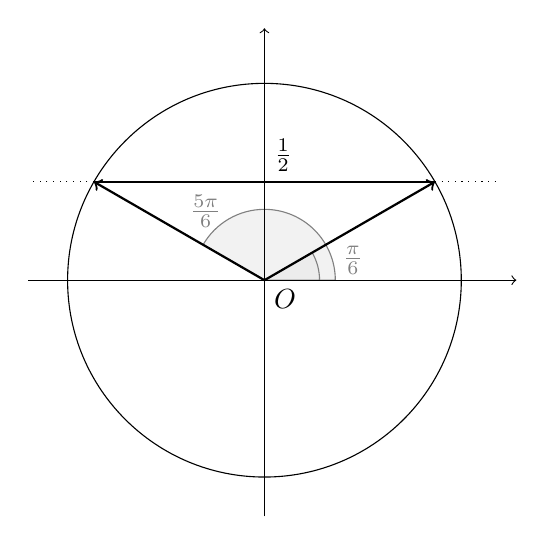
\begin{tikzpicture}[scale=1]
	            % Kružnice
	            \draw (0,0) circle (2.5cm);

	            % Počátek
	            \node[below right] at (0,0) {$O$};

	            % Úhly a jejich výplně
	            % Úhel alpha (červený, 0° až 25°)
							\filldraw[gray!10, draw=gray] (0,0) -- (0:0.9) arc (0:150:0.9) -- cycle;
							\node[gray] at (130.5:1.15) {$\frac{5\pi}{6}$};

	            \filldraw[gray!15, draw=gray] (0,0) -- (0:0.7) arc (0:30:0.7) -- cycle;
	            \node[gray] at (12.5:1.15) {$\frac{\pi}{6}$};

	            % Úhel beta (modrý, 90° až 60°)
	            %\filldraw[blue!15, draw=blue] (0,0) -- (90:0.8) arc (90:60:0.8) -- cycle;
	            %\node[blue] at (75:1.05) {$\beta$};

	            % Úhel phi (šedý, 25° až 60°)
	            %\filldraw[gray!30, draw=black] (0,0) -- (25:0.8) arc (25:60:0.8) -- cycle;
	            %\node at (42.5:1.05) {$\varphi$};

	            % Vektory a tečkovaná prodloužení
							\draw[thick] (150:2.5) -- (30:2.5);
							\node[anchor= south west] at (0,1.25) {$\frac{1}{2}$};
	            \draw[->, thick] (0,0) -- (30:2.5);
							\draw[->, thick] (0,0) -- (150:2.5);
	            \draw[dotted] (30:2.5) -- (3,1.25);
							\draw[dotted] (150:2.5) -- (-3,1.25);

	            %\draw[->, thick, blue] (0,0) -- (60:2.5) node[right] {$\vec{v}$};
	            %\draw[dotted] (60:2.5) -- (60:3.2);

							% Souřadnicové osy
	            \draw[->] (-3,0) -- (3.2,0);
	            \draw[->] (0,-3) -- (0,3.2);
	        \end{tikzpicture}
					\caption{Řešení příkladu \ref{gonrce1}}
\end{figure}
Je tedy
$$P = \left\{\frac{\pi}{6}+2k \pi; k \in \mathbb Z\right\} \cup \left\{\frac{5\pi}{6}+2k \pi; k \in \mathbb Z\right\}.$$
\end{reseni}

\begin{priklad}\label{gonrce2}
V $\mathbb R$ řešte rovnici $\tg x = -\sqrt{3}. $
\end{priklad}

\begin{reseni}
Z náčrtku grafu a základních hodnot funkce $\tg$ vidíme $x_1=-\frac{\pi}{3}+k\pi$, tedy
$$P = \left \{-\frac{2\pi}{3}+k\pi; k \in \mathbb Z\right\}.$$
\begin{comment}
\begin{figure}
	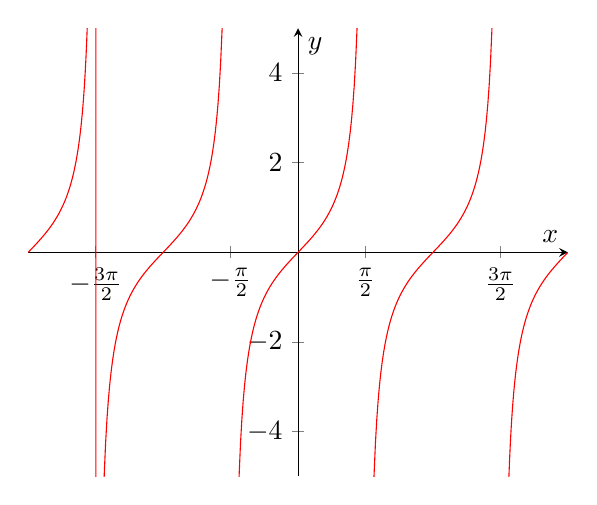
\begin{tikzpicture}
	\begin{axis}[
		axis lines=middle,
		xlabel=$x$, ylabel=$y$,
		xmin=-2*pi, xmax=2*pi,
		ymin=-5, ymax=5,
		trig format plots=rad,
		xtick={-1.5*pi, -0.5*pi, 0.5*pi, 1.5*pi},
		xticklabels={$-\frac{3\pi}{2}$, $-\frac{\pi}{2}$, $\frac{\pi}{2}$, $\frac{3\pi}{2}$}
	]
		% Define a small offset to avoid infinity
		\def\offset{0.01}

		% Plot segments with shrunk domains
		\addplot[red, domain=-2*pi:-1.5*pi+\offset, samples=100] {tan(x)};
		\addplot[red, domain=-1.5*pi+\offset:-0.5*pi-\offset, samples=100] {tan(x)};
		\addplot[red, domain=-0.5*pi+\offset:0.5*pi-\offset, samples=100] {tan(x)};
		\addplot[red, domain=0.5*pi+\offset:1.5*pi-\offset, samples=100] {tan(x)};
		\addplot[red, domain=1.5*pi+\offset:2*pi, samples=100] {tan(x)};
	\end{axis}
\end{tikzpicture}
	\caption{Řešení příkladu \ref{gonrce2}}
\end{figure}
\end{comment}
\end{reseni}

\begin{priklad}\label{gonrce3}
V $\mathbb R$ řešte nerovnici $\sin x \geq \frac{\sqrt{2}}{2}.$
\end{priklad}

\begin{reseni}
	Z náčrtku jednotkové kružnice a základních hodnot funkce $\sin$ vidíme
	$$P = \bigcup\limits_{k \in \mathbb Z} \left<\frac{\pi}{4}+ 2k\pi,\frac{3\pi}{4}+ 2k\pi \right>.$$
	\begin{comment}
	\begin{figure}[!ht]
		\centering
		        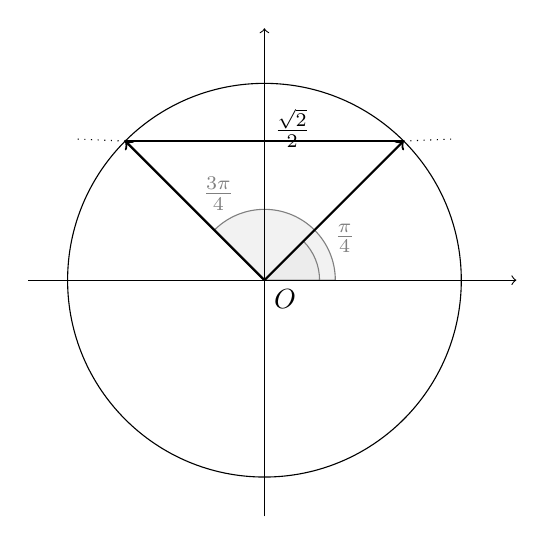
\begin{tikzpicture}[scale=1]
		            % Kružnice
		            \draw (0,0) circle (2.5cm);

		            % Počátek
		            \node[below right] at (0,0) {$O$};

		            % Úhly a jejich výplně
		            % Úhel alpha (červený, 0° až 25°)
								\filldraw[gray!10, draw=gray] (0,0) -- (0:0.9) arc (0:135:0.9) -- cycle;
								\node[gray, yshift=3pt] at (120.5:1.15) {$\frac{3\pi}{4}$};

		            \filldraw[gray!15, draw=gray] (0,0) -- (0:0.7) arc (0:45:0.7) -- cycle;
		            \node[gray] at (27.5:1.15) {$\frac{\pi}{4}$};

		            % Úhel beta (modrý, 90° až 60°)
		            %\filldraw[blue!15, draw=blue] (0,0) -- (90:0.8) arc (90:60:0.8) -- cycle;
		            %\node[blue] at (75:1.05) {$\beta$};

		            % Úhel phi (šedý, 25° až 60°)
		            %\filldraw[gray!30, draw=black] (0,0) -- (25:0.8) arc (25:60:0.8) -- cycle;
		            %\node at (42.5:1.05) {$\varphi$};

		            % Vektory a tečkovaná prodloužení
								\draw[thick] (135:2.5) -- (45:2.5);
								\node[yshift = 4pt, anchor=west] at (0,0.717*2.5) {$\frac{\sqrt{2}}{2}$};
		            \draw[->, thick] (0,0) -- (45:2.5);
								\draw[->, thick] (0,0) -- (135:2.5);
		            \draw[dotted] (45:2.5) -- (2.4,0.717*2.5);
								\draw[dotted] (135:2.5) -- (-2.4,0.717*2.5);

		            %\draw[->, thick, blue] (0,0) -- (60:2.5) node[right] {$\vec{v}$};
		            %\draw[dotted] (60:2.5) -- (60:3.2);

								% Souřadnicové osy
		            \draw[->] (-3,0) -- (3.2,0);
		            \draw[->] (0,-3) -- (0,3.2);
		        \end{tikzpicture}
						\caption{Řešení příkladu \ref{gonrce3}}
	\end{figure}
\end{comment}
\end{reseni}
